\section{Technology Assessment}
\label{sec:technology}

Introduce in (sufficient) depth the key concepts and architecture of the chosen software technology. As part of this, you may consider using a running example to introduce the technology.

This part and other parts of the report probably need to refer to
figures. Figure~\ref{fig:framework} from \cite{brown:96} just
illustrates how a figure can be included in the report.

\begin{figure}[thb]
	\centering
	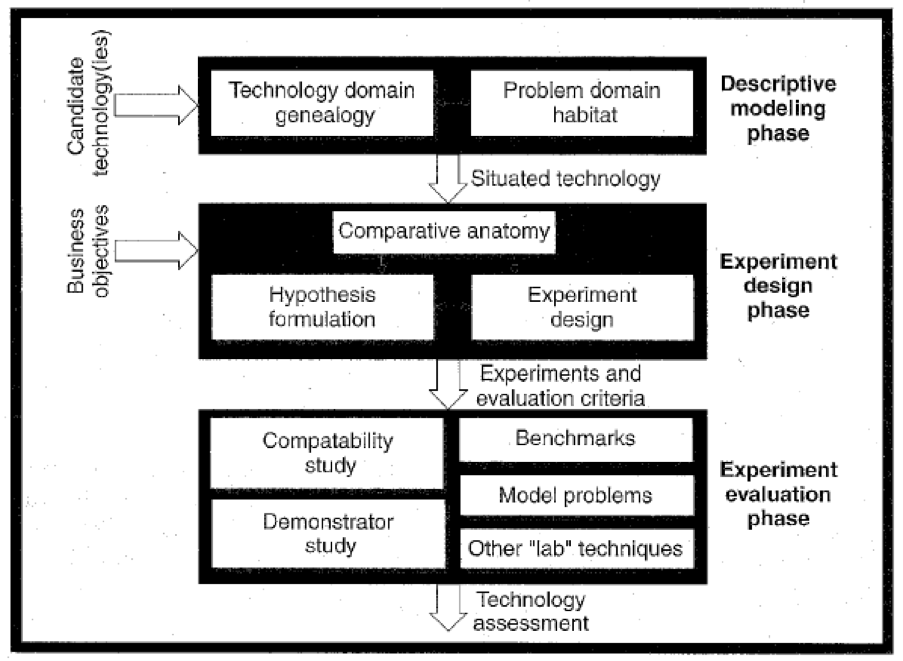
\includegraphics[scale=0.5]{figs/framework.png}
	\caption{Software technology evaluation framework.}
	\label{fig:framework}
\end{figure}

\subsection{Descriptive Modeling}

Write about where the technology comes from, its history, its context, and what problem it solves.
Consider drawing a graph like in \cite{brown:96}.

\subsection{Experiment Design}

\subsubsection*{Hypotheses}

\begin{enumerate}
    \item \textbf{Security Improvement Hypothesis}: OAuth 2.0 will provide improved security over traditional username and password authentication by reducing the need to store sensitive user credentials directly within the app's database.

    \item \textbf{User Experience Improvement Hypothesis}: OAuth 2.0 will enhance the user experience by simplifying the login process, allowing users to log in with existing accounts from trusted providers like Google or GitHub.
\end{enumerate}

\subsubsection*{Experiment Design to Support or Reject Hypotheses}

\begin{enumerate}
    \item \textbf{Testing the Security Improvement Hypothesis}

    \begin{itemize}
        \item \textbf{Experiment}: Conduct a security risk analysis of both authentication methods. For the traditional method, store user credentials in a local database, then perform a simulated data breach to see how each system protects user information. Measure the impact of using OAuth 2.0, which keeps sensitive data with the provider, thereby limiting the risk of exposure in case of a breach.
        \item \textbf{Expected Outcome}: If OAuth 2.0 significantly reduces the risk of data exposure, the hypothesis will be supported.
    \end{itemize}

    \item \textbf{Testing the User Experience Improvement Hypothesis}

    \begin{itemize}
        \item \textbf{Experiment}: Implement both authentication methods (traditional and OAuth 2.0) and conduct a usability test with a sample group of users. Track metrics such as the time taken to complete the login process, user feedback, and abandonment rate (users who quit during signup).
        \item \textbf{Expected Outcome}: If OAuth 2.0 shows a lower abandonment rate and faster login times, it supports the hypothesis that OAuth improves user experience.
    \end{itemize}
\end{enumerate}

\subsection{Experiment Evaluation}

Write about the results of your experiments, either via personal experience reports, quantitative benchmarks, a demonstrator case study, or a combination of multiple approaches.

For some reports, you may have to include a table with experimental
results or other kinds of tables that, for instance, compare
technologies. Table~\ref{tab:results} gives an example of how to create a table.

\begin{table}[bth]
	\centering
	\begin{tabular}{llrrrrrr}
		Config & Property & States & Edges & Peak & E-Time & C-Time & T-Time
		\\ \hline \hline
		22-2 & A   &    7,944  &   22,419  &  6.6  \%  &  7 ms & 42.9\% &  485.7\% \\
		22-2 & A   &    7,944  &   22,419  &  6.6  \%  &  7 ms & 42.9\% &  471.4\% \\
		30-2 & B   &   14,672  &   41,611  &  4.9  \%  & 14 ms & 42.9\% &  464.3\% \\
		30-2 & C   &   14,672  &   41,611  &  4.9  \%  & 15 ms & 40.0\% &  420.0\% \\ \hline
		10-3 & D   &   24,052  &   98,671  & 19.8  \%  & 35 ms & 31.4\% &  285.7\% \\
		10-3 & E   &   24,052  &   98,671  & 19.8  \%  & 35 ms & 34.3\% &  308.6\% \\
		\hline \hline
	\end{tabular}
	\caption{Selected experimental results on the communication protocol example.}
	\label{tab:results}
\end{table}
